
\chapter{虚拟机实现}
\label{ch:vm impl}

在这一章节中,主要讲解如何去具体实现一个虚拟机。在解释器组成章节中,提到了一个语言运行需要两个上下文,其中一个称之为环境,另一个称之为控制上下文。环境负责管理变量并为程序提供词法作用域。控制上下文为程序提供函数调用所需要的状态管理功能。但是这两个上下文之间又不是完全相互独立的。在scheme中,函数被创建的时会捕获函数创建时所在的作用域。这时我们通常不称之为函数,而是称之为闭包。在本章节中,主要便是描述如何围绕这两个上下文去设计虚拟机的模型,包括寄存器以及指令集。

EdenApple虚拟机实现模型主要基于Kent. R Dybvig的论文\cite{dybvig87timpl}中的heap-based model。接下来首先虚拟机的运行模型以及管理状态所需的寄存器,然后给出该虚拟机的指令集以及具体的语句如何翻译到这些指令。

在实现语言的选择上使用了JavaScript,并使用了ES6的新特性。使用JS是为了简单方便,能够比较方便的描述出EdenApple的实现,因此能够专注于模型的设计。

\section{虚拟机模型}

首先介绍环境的结构。环境是管理变量以及词法作用域的一种结构。环境由帧组成。每一帧对应着一个具体的作用域,也就是说在每一帧中包含着所有该作用域中变量的名称到值的映射。同时,每一帧都会包含一个指向其父作用域的一个指针。通过这种控制结构,便能以一种层次化的结构管理程序运行的所有变量。

在图\ref{fig:env sample}中以图形的方式展示了环境的结构。

\begin{figure}
\begin{center}
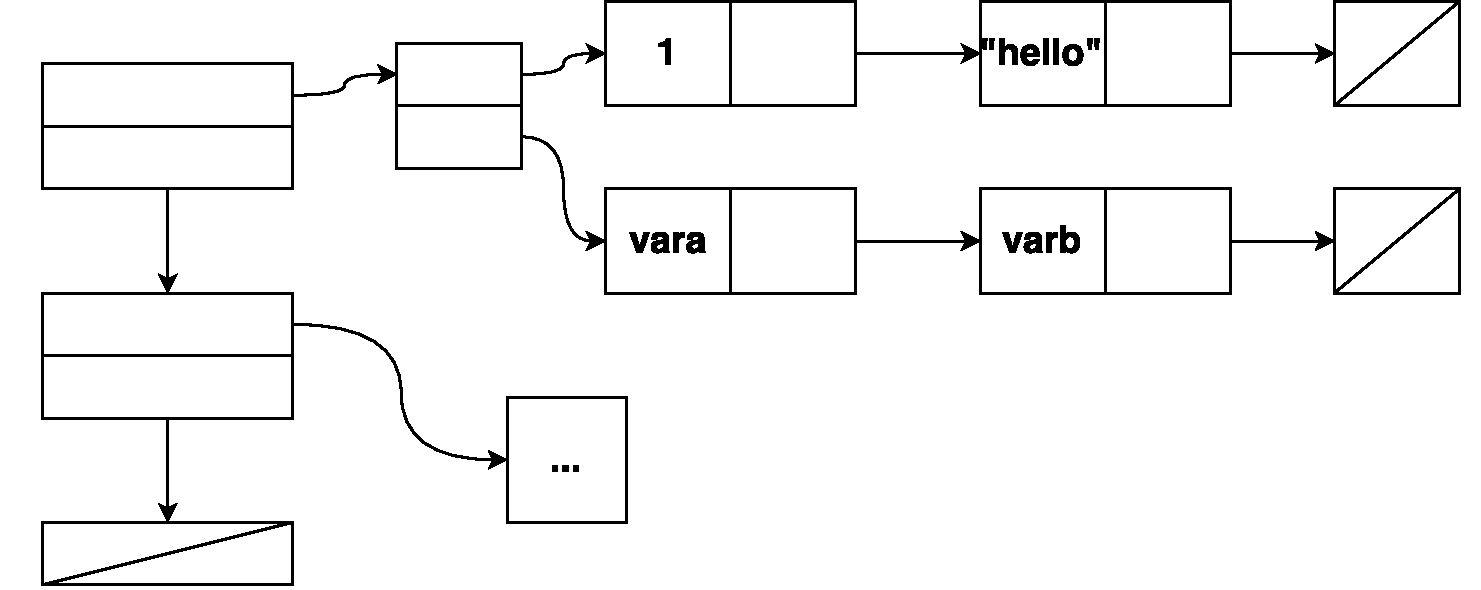
\includegraphics[width=\textwidth]{environment}
\end{center}
\caption{环境图形示例}
\label{fig:env sample}
\end{figure}

控制栈保存程序的执行状态,当程序的执行过程中,转而调用另一个函数时,旧的函数的执行状态需要被保存,这种信息保存在一个控制帧中。因此,一级一级函数的调用过程,便会构造出函数调用栈。在每一个帧中,需要保存,环境,下一条指令,函数调用的参数,以及上一级控制帧。

控制栈的结构可以参考图\ref{fig:control stack sample}。

\begin{figure}
\begin{center}
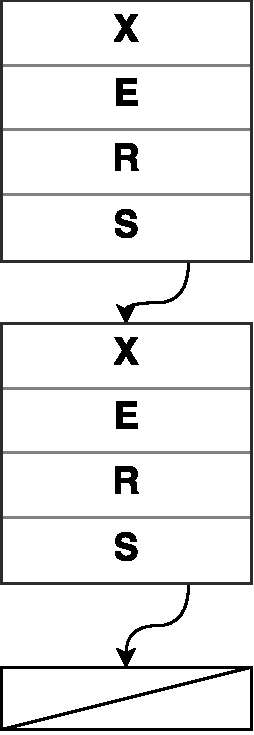
\includegraphics[height=200pt]{controlstack}
\end{center}
\caption{控制栈图形示例}
\label{fig:control stack sample}
\end{figure}

这里需要特别说明,函数调用的参数如何保存。一个函数的参数可能是一个,也可能是多个,而且在获取参数值时,通常需要对另一个表达式求值。因此需要一种列表结构来保存函数的参数值。在论文中,将这种特殊的结构称之为rib,并为此专门分配了一个的寄存器。

在一个机器中,我们通常以寄存器来维护程序运行的当前状态。本虚拟机使用类似secd机的虚拟机结构。具体的,有五个专用寄存器。

\begin{itemize}
\item \texttt{a} --- 累加寄存器,保存一个指令运行的结果,
\item \texttt{x} --- 指令寄存器,保存下一步执行的指令,
\item \texttt{e} --- 环境寄存器,保存当前的环境帧,
\item \texttt{r} --- 参数寄存器,保存函数调中参数的值,
\item \texttt{s} --- 控制栈寄存器,保存当前控制栈中栈顶的帧。
\end{itemize}

对比这个寄存器结构与上面所述的控制帧结构,可以发现,控制帧的创建实质上是对寄存器的一个快照。

\section{指令集}

EdenApple虚拟机中的指令集仅提供对程序运行状态的管理,在x86这些实际的机器中必然要提供数值计算的指令集。但是在此,这些操作以另一种方式提供。所有的这些数值操作,可以看作是以这些数值为参数的函数,又因为在scheme中,函数是一等公民,于是便可以将这些函数作为基本操作放入到全局作用域中。这样,虚拟机这需要提供完成核心功能所需要的指令即可。

EdenApple提供的指令集如下:

{
\singlespacing
\fontsize{10}{10}
\ttfamily
\begin{itemize}
\item halt
\item constant
\item refer
\item extend
\item assign
\item test
\item close
\item conti
\item nuate
\item frame
\item argument
\item apply
\item return
\end{itemize}
}

%指令中有,专门处理环境里有专门处理控制的,其中的环境操作一般是,跟控制站的操作是符合的,比如说函数调用,
%有简单往复杂,let,call。这两个指令组成操作环境的扩展操作,call指令也扩展了调用栈。Set,define指令也操作了环境,let和define的不同,define翻译成letrec,letrec与let不同在于letrec定义的数据可以是互递归的。

最基本的,\texttt{constant}指令将一个值存入寄存器a。\texttt{refer}指令从环境(e寄存器)中查找所给的名称对应的值放入a。

\texttt{extend}指令创建一个新的作用域。对应的是scheme中的\texttt{let}表达式。\texttt{extend}指令使用r寄存器中都值以及所给的名称列表创建新的一个环境帧,指定其父级上一级环境为e寄存器中的值。但是let表达式的编译过程还需要更多的处理操作,这些操作与函数调用语句的翻译中的操作类似,更多的细节将在\nameref{sec:vm impl:compile}一节中描述。事实上let语句完全可以看作是定义一个临时的函数并立即调用的操作,比如示例\nameref{lst:let-lambda-sample},但是函数调用编译出的指令序列会包含一些不必要的操作,因此额外提供作用域扩展的指令。

\begin{code}
\begin{minted}{scheme}
(let ([a 1]
      [b 2])
  (+ a b))
;; 等价于
((lambda (a b)
   (+ a b))
 1 2)
\end{minted}
\caption{let的lambda等价表示}
\label{lst:let-lambda-sample}
\end{code}

多数的操作都可以用lambda演算表示,变量的定义可以通过lambda函数调用时绑定变量实现(反过来,传参也可以看作是本地变量定义),甚至递归函数可以通过单纯的lambda演算表示,不动点组合子Y便是通过纯lambda演算实现递归的一种方式。

对参数求值时也需要一种结构,在上面曾经提到过函数调用的过程通常伴随着对参数表达式求值的求值。在这种情况下,需要将参数表达式所求的值临时保存。这就是\texttt{argument}指令的用处,在\nameref{sec:vm impl:compile}会详细讲解函数调用语句如何编译。

\texttt{assign}指令是\texttt{set!}语句的实现,\texttt{assign}指令将从环境中找到对应的变量,并将寄存器a中的替换。

\texttt{apply}指令应用一个函数调用,首先,他会将寄存器r中的值与所给的名称列表结合扩展当前的环境。这一步与上述的\texttt{extend}指令操作类似。同时,\texttt{apply}指令会将闭包中的环境替换到寄存器e,将闭包中的函数指令放入到寄存器x中。

\texttt{return}指令是一个函数指令序列的最后一个,该指令从控制栈中pop一层帧,并将该帧中的数据恢复到寄存器。

\texttt{close}指令创建一个闭包,若你具有c语言背景,可能会奇怪,在c中,函数本身只是一个地址,为什么需要一个额外的指令创建?事实上,函数的指令部分当然不需要额外的指令操作,此处创建的函数闭包除了指令本身信息和参数名称列表以外,还包括了函数创建时所在的作用域,也就是e寄存器的数据。

\texttt{conti}指令创建一个continuation,在这个continuation随后被调用时,会执行nuate指令恢复到他被创建时的寄存器环境。

\section{编译}
\label{sec:vm impl:compile}

在EdenApple中的基本语法关键字包括\texttt{define, let, lambda, if, call/cc},这些关键字代表了他们所对应的语法式,除此之外,一个普通的列表被当作是一次函数调用。一个非symbol的atom被当作一个常量,一个symbol被当作变量引用。

这样子,如果不考虑优化的话,翻译便非常直接了,常量翻译成\texttt{constant}指令,变量引用翻译成\texttt{refer}指令,等等。

这里需要额外讨论的是函数调用以及\texttt{call/cc}。

函数调用是一个复杂的过程,首先,需要对每一个参数求值,在每一次求值之后插入一条\texttt{argument}指令将参数存入到寄存器r中。随后对所需的函数求值,严格来说,是对列表中的第一项求值,这个值应当是闭包类型。之后便是\texttt{apply}指令。

为了支持尾递归,在函数调用表达式被编译时还要判断该语句是否处于尾递归位置,若不是处于尾递归位置,还需要在对参数求值之前插入一条\texttt{frame}指令创建一个新的控制帧。

\texttt{call/cc}语句指令创建了一个continuatin,\texttt{call/cc}的唯一参数是一个接收一个值的函数。因此,call/cc翻译的指令序列是\texttt{conti argument <eval arg> apply},同样的,作为一个带\texttt{argument}和\texttt{apply}的序列,需要做尾递归检查,并在非尾递归时在序列前端插入\texttt{frame}指令。

另外值得一提的是\texttt{define}语句,\texttt{define}语句可以看作是\texttt{letrec}语句的语法糖,在编译时需要做更多的上下文检查和分析。

在EdenApple中,实现了一个基本的\texttt{letrec},但是为了简单与专注,并没有实现\texttt{define}语法糖。

\section{基本操作}

一个数据结构需要相对应的操作才能体现出其作用,比如数若是没有加减乘除操作,便无法体现数的作用。在EdenApple中,类型信息保存在数据一边,变量无需显示的标注类型,因此对外需要暴露的是与各种类型配套的基本操作。
在EdenApple中,内置了如下这些基本操作,如果将全局看作是一级作用域,那么在此处,这些基本操作被放在了零级作用域,也就是全局作用域的父作用域中。
在EdenApple中,有如下基本操作:

\begin{enumerate}
\item 数据类型 (\texttt{symbol? number? boolean? string? pair? null? procedure?})
\item 列表操作 (\texttt{cons car cdr})
\item 数值操作 (\texttt{+ - * / mod})
\item 逻辑计算 (\texttt{< <= = >= >})
\item IO操作 (\texttt{display newline})
\item 其他 (\texttt{list?})
\end{enumerate}

这些基本操作完全通过宿主语言实现,在其他语言中,这些基本操作,比如\texttt{+ - * / > <}会被当作是操作符,本身作为语言的一部分,并且在编译时也会直接翻译到对应的指令。但是在scheme中,他们也是一等函数,这在带来操作方便以及一致的语义的同时也意味着无法简单的将他们翻译成对应的指令,因此也造成了性能上的一些损失。